\documentclass{higrep}
\usepackage[hyphens]{url} % you can use \url{www.myurl.com} in your text
                          % long urls will be broken over lines using hyphens
\usepackage{listings} % useful for formatting program listings
\usepackage{xspace}  % used for conditionally inserting spaces
\usepackage{cite} % used for multiple citations

% some typical settings for listings
\lstset{
    basicstyle=\footnotesize,
    numberstyle=\tiny,
    numbers=left,
    numberstyle=\tiny,
    stepnumber=1,
    numbersep=5pt,
    tabsize=2,
    showstringspaces=false,
    aboveskip=\smallskipamount,
    belowskip=\smallskipamount
    %aboveskip=\medskipamount,
    %belowskip=\medskipamount
}

% here is an example of defining a new language for listings
\lstdefinelanguage{pseudo}{
    sensitive=true, % Case sensitive identifiers
    morecomment=[l]{\#}, % Line-based comment character
    %morestring=[b]&, % String character
    morekeywords= {
		function,
		repeat,
		until,
		for,
		loop,
		foreach,
		while,
		if,
		else,
		end,
		equals,
		add,
		remove,
		return,
		get,
		set,
		parse,
		call,
		increment
	},
	commentstyle=\color[rgb]{.600,.600,.600}, % grey comments
}

% these are useful for referring to sections, listings, figures ...
\newcommand{\sectionref}[1]{Section~\ref{#1}}
\newcommand{\secref}[1]{Sec.~\ref{#1}}
\newcommand{\lstref}[1]{Listing~\ref{#1}}
\newcommand{\figureref}[1]{Figure~\ref{#1}}
\newcommand{\figref}[1]{Fig.~\ref{#1}}
\newcommand{\tableref}[1]{Table~\ref{#1}}
\newcommand{\equationref}[1]{Equation~\ref{#1}}

% you can define some commonly used commands here ... 
\newcommand{\parfor}{\texttt{parfor}\xspace}
\newcommand{\mclab}{{\sc M}c{\sc Lab}\xspace}
\newcommand{\matlab}{{\sc Matlab}\xspace}
\newcommand{\smatlab}{{\sc Matlab}}
\newcommand{\kw}[1]{\texttt{#1}}

\def\code#1{\texttt{#1}}

% to add margin note you can use \mynote, and then remove then by 
% commenting out the first option and uncommenting the second option
\newcommand{\mynote}[1]{\marginpar{\tiny{#1}}}
%\newcommand{\mynote}[1]{}



% -------------------------- All the Front matter info ---------------
\frontmatter
% uncomment and put a different group name, if you are not HIG
%\laboratory{Your Group Name Here}

% pick your report number, based on the year and the next available
% report #
\reportnum{HIG-2017-01 Anna Jolly}

% choose one of the following,  or insert your own.
%\program{COMP 396}
\program{MDPH 396}
%\program{COMP 400}
%\program{COMP 401}
%\program{}

% the default distribution is for public release, uncomment and edit 
% following line if you have a different distribution restriction.
% \distribution{Available for the HIG group only.}

% you must give a title
\title{Physician-Created Questionnaires in the Mobile Application Opal}

% a subtitle is optional, delete if you don't want one
%\subtitle{Software Architecture}

% You must put the date, you may not need the revised part
%\date{March 2017 \\Revised March 2017}
\date{March 2017}

%list authors, each author has an affiliation, which can be the address
%or other info like e-mail  as below

\author{Anna Jolly}

\affiliation{School of Computer Science\\
  McGill University, Montreal\\
  \texttt{anna.jolly@mail.mcgill.ca}}

% this is the artwork for the cover, you can change it, or 
% comment it out
\coverart{Images/cancercentre}

% put the type of report here
\reporttype{MDPH 396 Final Report}

% you can put some additional info for title page
\additionalinfo{Supervised by:  John Kildea, Medical Physics}
%\additionalinfo{Supersedes HIG-2014-02}

\begin{document}

\begin{abstract}
Patient-reported outcomes (PROs) are a valuable asset during a patient's cancer treatment. Having patients fill out PRO questionnaires in between clinical visits allows physicians to better monitor their patients. Opal, a mobile oncology application, provides standardized PRO questionnaires to patients when they check-in for their clinical visits. However, in the current version of Opal, physicians have little control over the questions that compose the questionnaires that are sent to their patients. This project addresses this issue via the implementation of a web application tailored to physicians that allows them to create and maintain questionnaires. The app enables physicians to access public standardized libraries of questions and questionnaires, and allows them to create their own questions and questionnaires, as well as access their patients' completed questionnaires. This report details the design and implementation of the application.
\end{abstract}

\disclaimer{}
% uncomment the following if you want disclaimer - make 
%\disclaimer{Insert your disclaimer here.}

\maketitle

\tableofcontents

\listoffiguresandtables

% here are some chapters that are part of the preamble part of the
% report,  examples of what you might put are Acknowledgements or Tables
% of Abbreviations or terms,  or a French version of the abstract.

\chapter{Acknowledgements}

First and foremost, I would like to thank my supervisor Dr. John Kildea for his continual guidance and critique throughout this project. I would also like to thank Prof. Laurie Hendren for her advice and enthusiasm during our weekly meetings and Dr. Tarek Hijal for his inspiring tour of radiation oncology. Lastly, I would like to thank Robert Maglieri, who was always there to help me when I needed it, and all the other students and developers for their insight.

\chapter{Abbreviations}

\begin{description}
\item [PRO]: Patient-reported outcome
\item [EHR]: Electronic health record
\item [Opal]: Oncology portal and application
\item [HIG]: Health Informatics Group
\item [MUHC]: McGill University Health Centre
\item [PRE]: Patient-reported experience
\item [MVC]: Model-View-Controller

\end{description}


% --------------------------  The main part of the report starts here 
\mainmatter

% you can put a label on chapters and sections and then use \ref{} to
% refer to the label.
\chapter{Introduction}

Patient-reported outcomes (PROs) are measurements of a patient's quality of life as reported by the patient. Between clinical visits, patients' symptoms and concerns often go unaddressed, and PROs are an efficient way of potentially identifying issues that need to be addressed with the patient's physician. The recent rise in the use of smartphones has paved the way for this new patient-physician communication to be integrated into electronic health records (EHR). Basch et al. showed numerous clinical benefits associated with the use of PROs in cancer care, including improved health-related quality of life and a decrease in the frequency of hospitalizations\cite{basch16}.

Opal is a mobile application for oncology patients developed by the Health Informatics Group (HIG) at the MUHC. Opal provides personalized information and data to patients at the MUHC, and is designed to allow patients to submit PRO data while they wait for their appointments.

The purpose of this project is to design a web application for physicians that enables them to access standardized questionnaires as well as design their own questionnaires for both clinical and research purposes. Physicians should be able to access PRO and patient-reported experience (PRE) libraries, create their own questionnaires and questions, and view their patients' answered questionnaires. These questionnaires will then be made available to patients on Opal. This project involves the design and implementation of the web application using AngularJS, PHP, and MySQL.

In \sectionref{Sec:RelatedWork} we briefly cover related work in the field of PRO software and in \sectionref{Sec:Background}, we introduce Opal and its current PRO interface. In \sectionref{Sec:DesignRequirements}, we outline the desired features and functionalities of the app. In \sectionref{Sec:SoftwareDesign}, we lay out the basic architecture of the app and discuss how the different components of the design interact and communicate with each other. We also provide justifications of the solutions employed to address the design requirements. Subsequently, \sectionref{Sec:Implementation} presents the end result of the project as it stands, with screenshots to demonstrate the app, its layout, and its functionalities. Lastly, in \sectionref{Sec:DiscussionAndFutureWork}, we discuss the challenges of the project and what remains to be done in the future, and in \sectionref{Sec:Conclusion}, we share some final thoughts with regards to the project.

\chapter{Related Work}\label{Sec:RelatedWork}

%Make sure you provide enough background and related work so that readers
%see where your work fits both within the local project, and within
%the global research area.    You need to be very careful to distinguish 
%background work on which you are building from your own contributions.
%When referring to papers or URLs, you can use \verb+\cite{label1}+ to
%entries in your \texttt{.bib} files.  For example, Lamport's book is
%a good reference for \LaTeX\cite{Lamport94}.    
%You can cite a bunch of papers in
%one like this.   You will find many other useful documents for
%\LaTeX\xspace
%and \LaTeX\xspace packages online\cite{Sommerfeldt07:Caption,Daly07:Natbib}.  

In the past few years, much research has been devoted to PROs and their efficiency and usefulness to both patients and physicians. Basch describes the challenges faced with incorporating PROs into patient care\cite{basch17} and enumerates the various advantages of PROs, including increased patient adherence to treatment, increased patient satisfaction with care, and decreased number of patient visits to the ER. Snyder et al. have developed User's Guide for implementing PRO assessment in clinical practice\cite{snyder12}.

As a result of this research, numerous medical institutions have begun to integrate PROs into their patient care, and many have turn to electronic systems to administer questionnaires to patients. Holzner et al. developed the Computer-based Health Evaluation Software (CHES), a software for administering PRO questionnaires, storing PRO data, and graphically presenting PRO results. CHES also includes a "Questionnaire Builder" for creating and editing questionnaires\cite{holzner12}. Duman-Lubberding et al. developed "OncoKompas", a three-part eHealth application that allows cancer survivors to monitor their quality of life via PROs, and then tailors feedback and advice bases on this data\cite{dl16}.

However, the vast majority of these softwares deal with making standardized questionnaires available to patients and collecting the patients' data. They rarely focus on the creation of the questionnaires themselves. This project aims to deal with this lack of versatility in questionnaire creation and editing, in addition to the usual issues of dealing with patient data.
 
\chapter{Background: Opal}\label{Sec:Background}

Opal is a mobile application that acts as a patient portal for radiation oncology patients. The app allows patients to access their personal health information. This includes appointment schedules, lab results, personalized educational material, radiotherapy treatment planning views, and more. The initial release of Opal had a basic PRO interface within the app that provided patients with the Edmonton Symptom Assessment System questionnaire weekly, and provided physicians with basic access to their patients' data\cite{us}. This project builds on top of this basic interface. Instead of standardized questionnaires, the patients will now be sent a wider variety of questionnaires that may be more tailored to them and their experiences.

\chapter{Design Requirements}\label{Sec:DesignRequirements}

The desired features and functionalities of the app are as follows:
\begin{itemize}
\item Implement a "tag"-based browsing system
\item Browse standardized PRO/PRE questionnaires
\item Create questionnaires using questions from PROM/PREM libraries
\item Create questionnaires using custom questions
\item Create custom answer types (multiple choice, checkboxes, etc.)
\item View, edit, and delete questionnaires
\item Tag questionnaires and questions with keywords
\item Push questionnaire to patients
\item View patients' questionnaire results
\item Share questionnaires and custom libraries with other physicians
\item Allow researchers to view anonymized results
\end{itemize}

\chapter{Software Design}\label{Sec:SoftwareDesign}

\section{Database Design}

To store all the questionnaire, question, and patient result data, we developed a custom database \textit{QuestionnaireDB}, managed via the MySQL database management system. The first step consisted of determining all the entities of the database, and how each entity relates to the others. \figureref{Fig:ER_Diagram} shows the entity-relationship diagram of \textit{QuestionnaireDB}. The basic structure consists of the following: libraries contain categories of question groupings, where a question grouping is either one question or in the case where several questions cannot be separated from each other, several questions. Questionnaires are made up of these question groupings, and each question has an associated answer type with it, under such categories as "Multiple Choice" and "Date", and each answer type is made up of several options that the patients may choose from. Tags are keywords that are associated with certain entities to facilitate a physician's browsing.

\begin{figure}[htbp]
  \centering
  \fbox{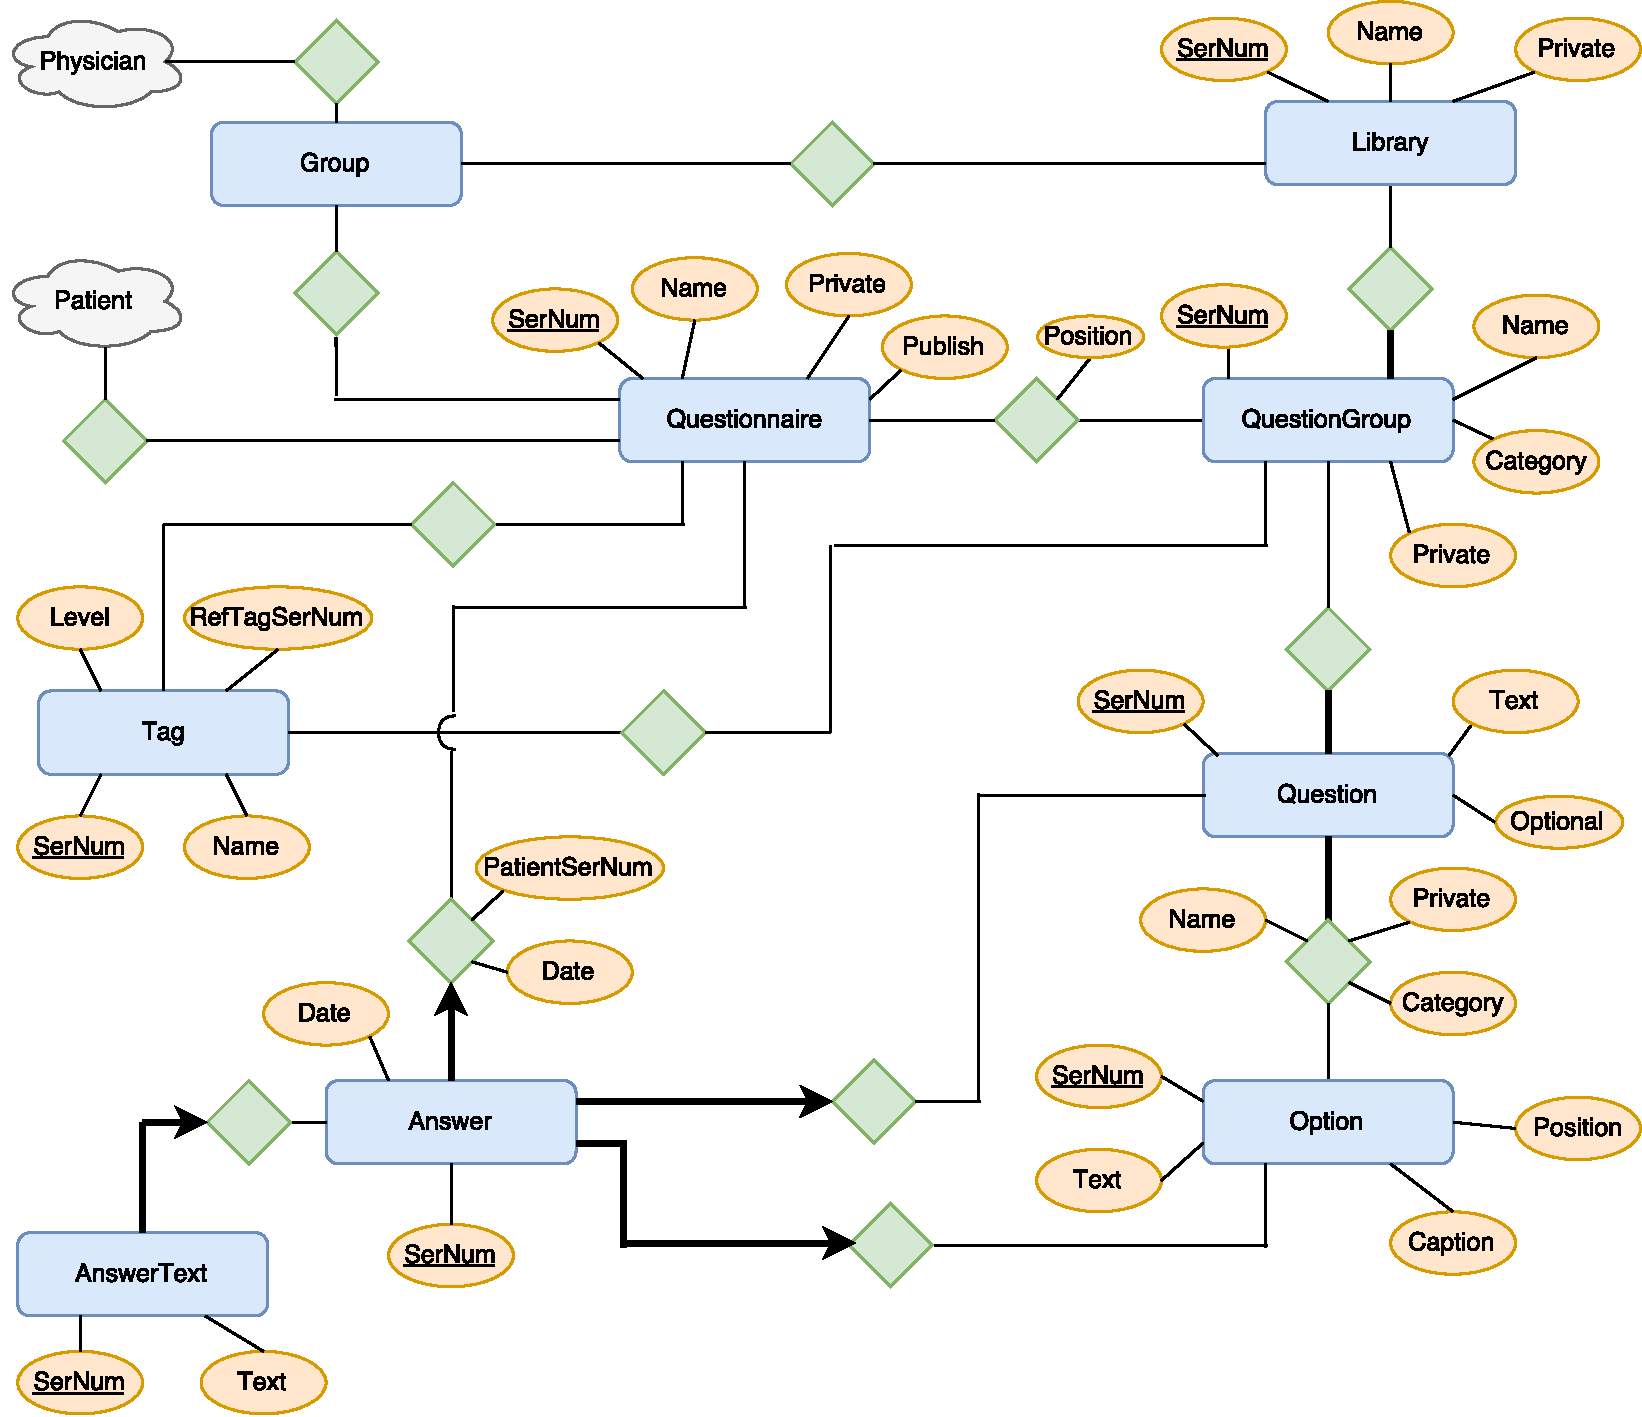
\includegraphics[scale=0.6]{Images/ER_Diagram.pdf}}
  \caption{Entity-relationship diagram of \textit{QuestionnaireDB}. The entities are in blue rectangles, their attributes in orange ellipses, and their relationships in green diamonds. The grey clouds indicate that Opal's database will link up there. A simple line represents a many-to-many relationship; a bolded line represents a participation constraint (the relationship must exist); an arrow represents a key constraint (at most one).} \label{Fig:ER_Diagram}
\end{figure}

\section{Interface Architecture}
The web application was developed using the Model-View-Controller (MVC) design pattern. The app uses AngularJS, a structural framework for dynamic web applications, in implementing this MVC design pattern. AngularJS enables dynamic views and provides two-way data binding as an automatic way of updating the view whenever the model changes and updating the model whenever the view changes. The result is a powerful and convenient environment. \figureref{Fig:MVC} shows the model-view-controller architecture of the web application. Two-way data binding links the model, view and controllers, and the controller communicates with \textit{QuestionnaireDB} using services that call PHP scripts. The PHP script is the method of direct communication with the database, selecting, inserting and deleting records from the database. The front-end of the app utilizes the framework Bootstrap in order to make the app responsive to various devices. The choice of a PHP server with a MySQL database for the back-end stems from the fact that MySQL is fast, reliable, and easy to use, PHP is designed for the web, and MySQL combined with PHP is cross-platform.

\begin{figure}[htbp]
  \centering
  \fbox{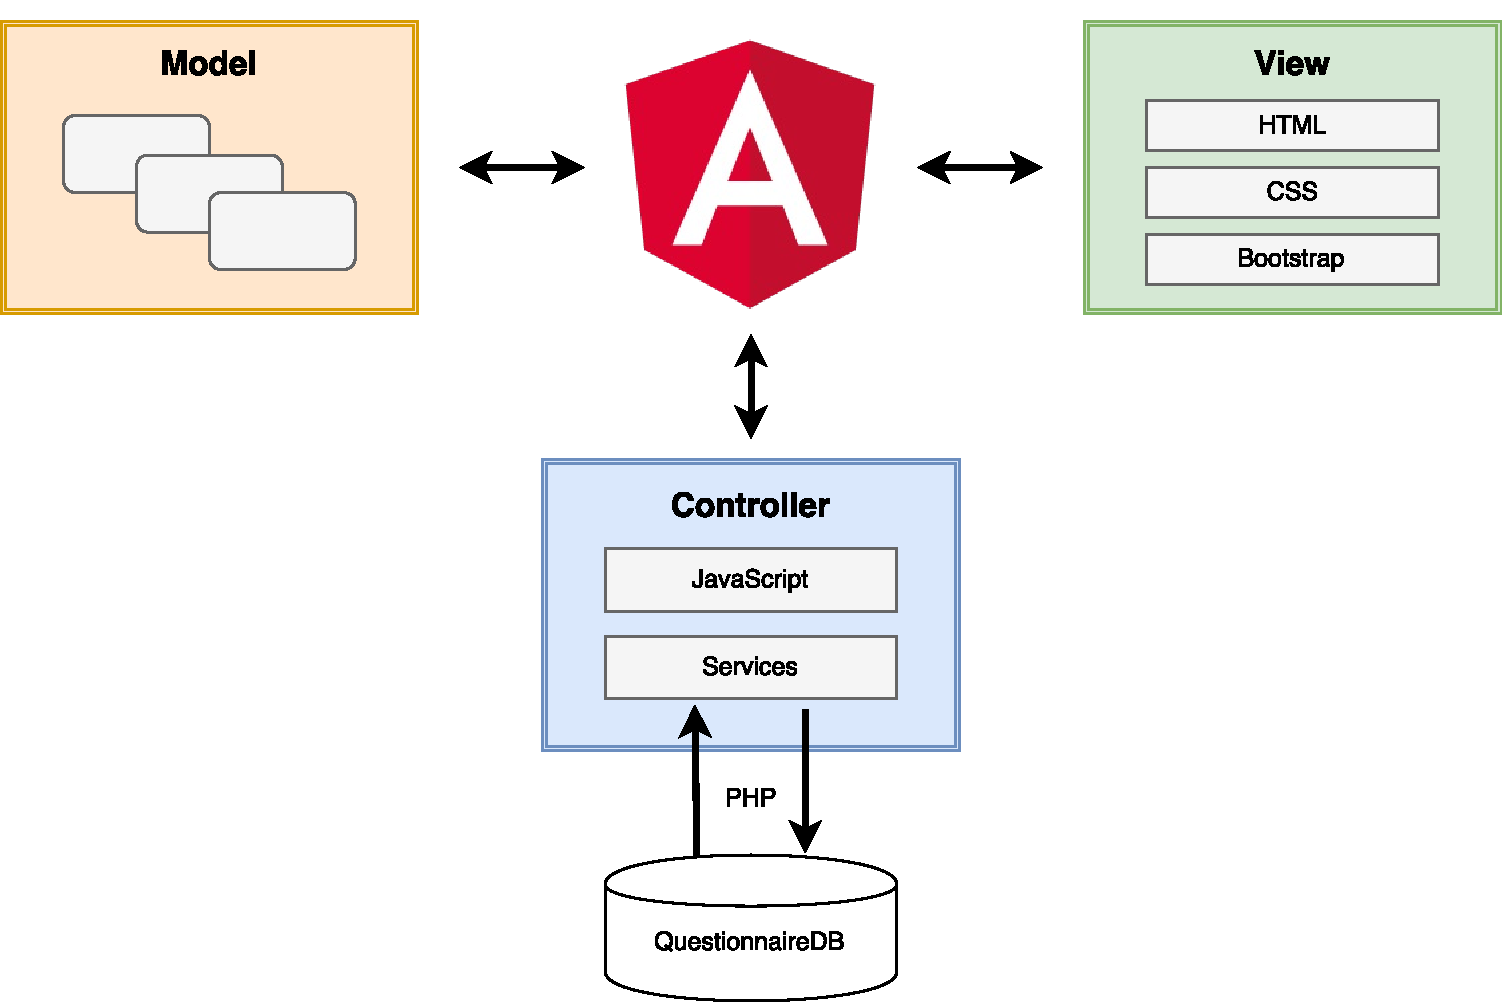
\includegraphics[scale=0.6]{Images/MVC.pdf}}
  \caption{The app's model-view-controller (MVC) architecture. The views, models, and controllers communicate via 2-way data binding, and the controller communicates with the database via PHP scripts.} \label{Fig:MVC}
\end{figure}

\chapter{Implementation}\label{Sec:Implementation}

A demo of the app prototype can be found at (COMING SOON).%%TODO.

Tables outlining the organization of the pages, their URLs, views and controllers can be found in \sectionref{Sec:Org} of the appendix.

The following section provides descriptions and screenshots of the app, showing the various features available to physicians. First off is the home menu as shown in \figureref{Fig:home} which can take the physician to the 4 main functionalities: creating questionnaires, viewing and editing questionnaires, viewing and editing the question bank, and viewing patients' questionnaire results.

\begin{figure}[htbp]
  \centering
  \fbox{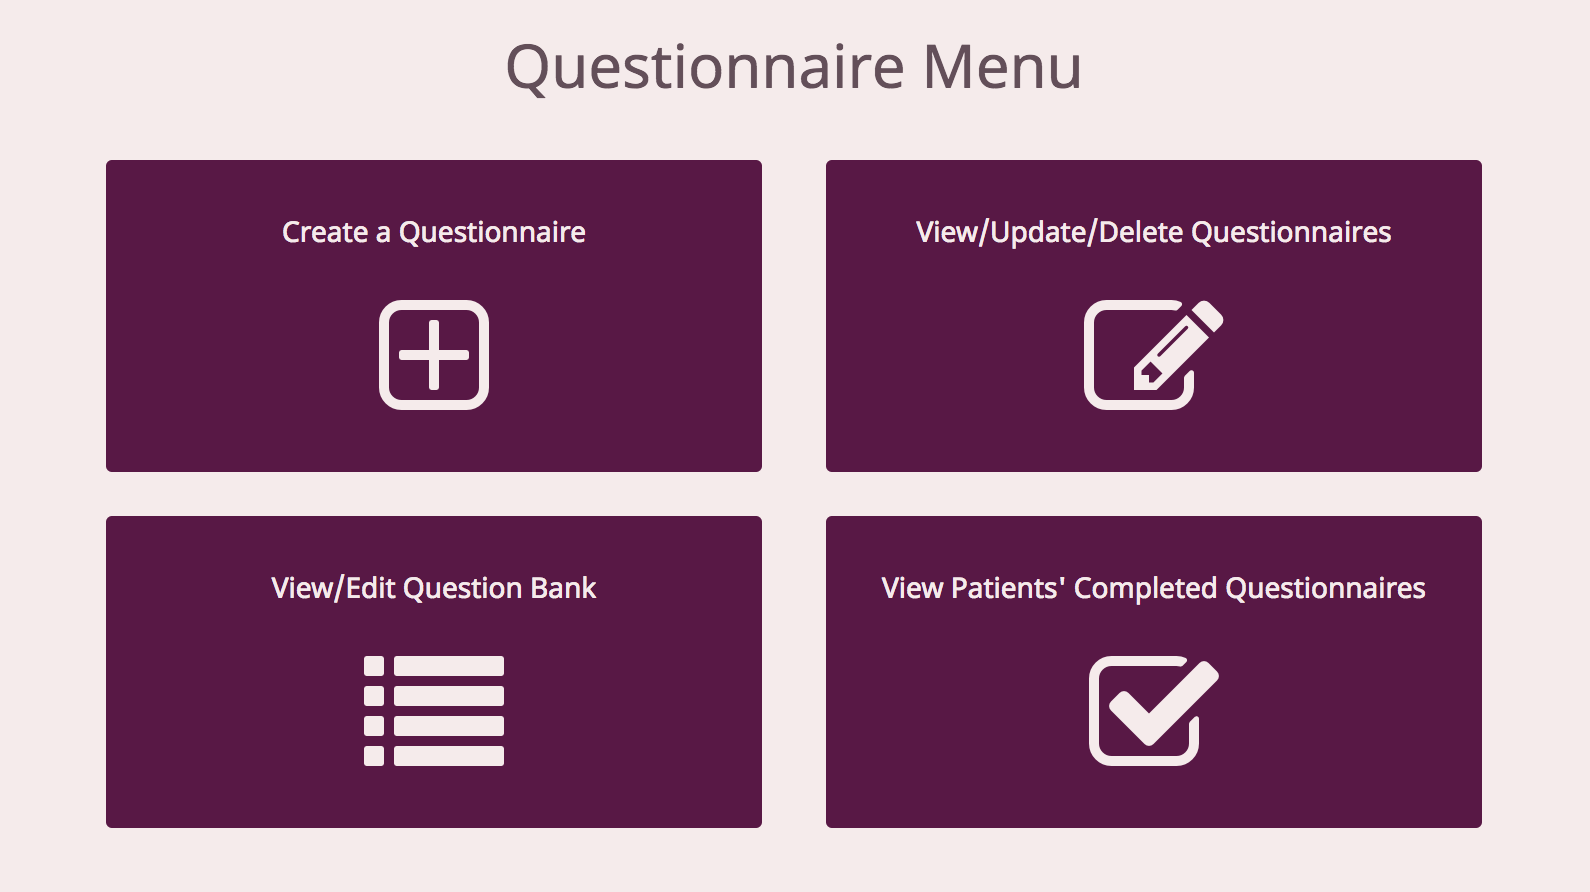
\includegraphics[scale=0.5]{Images/home.png}}
  \caption{Screenshot of the home menu of the app.} \label{Fig:home}
\end{figure}

\figureref{Fig:create} shows a first look at the questionnaire creation page. The questionnaire form requires the physician to specify if they would like the questionnaire to be private (only they can see and access it), or public (other physicians can also see and access it). The physician subsequently adds the question groupings that they want. As shown in \figureref{Fig:create_libraries}, the physician has the possibility of searching through all the public PROM/PREM libraries, as well as their own libraries and the libraries that they have been added to, and selecting the questions they want. A preview of the questionnaire shows up dynamically alongside the libraries. The physician may also target their search using tags. \figureref{Fig:create_tags} shows how this could be done to target libraries for prostate cancer, for example.

\begin{figure}[htbp]
  \centering
  \fbox{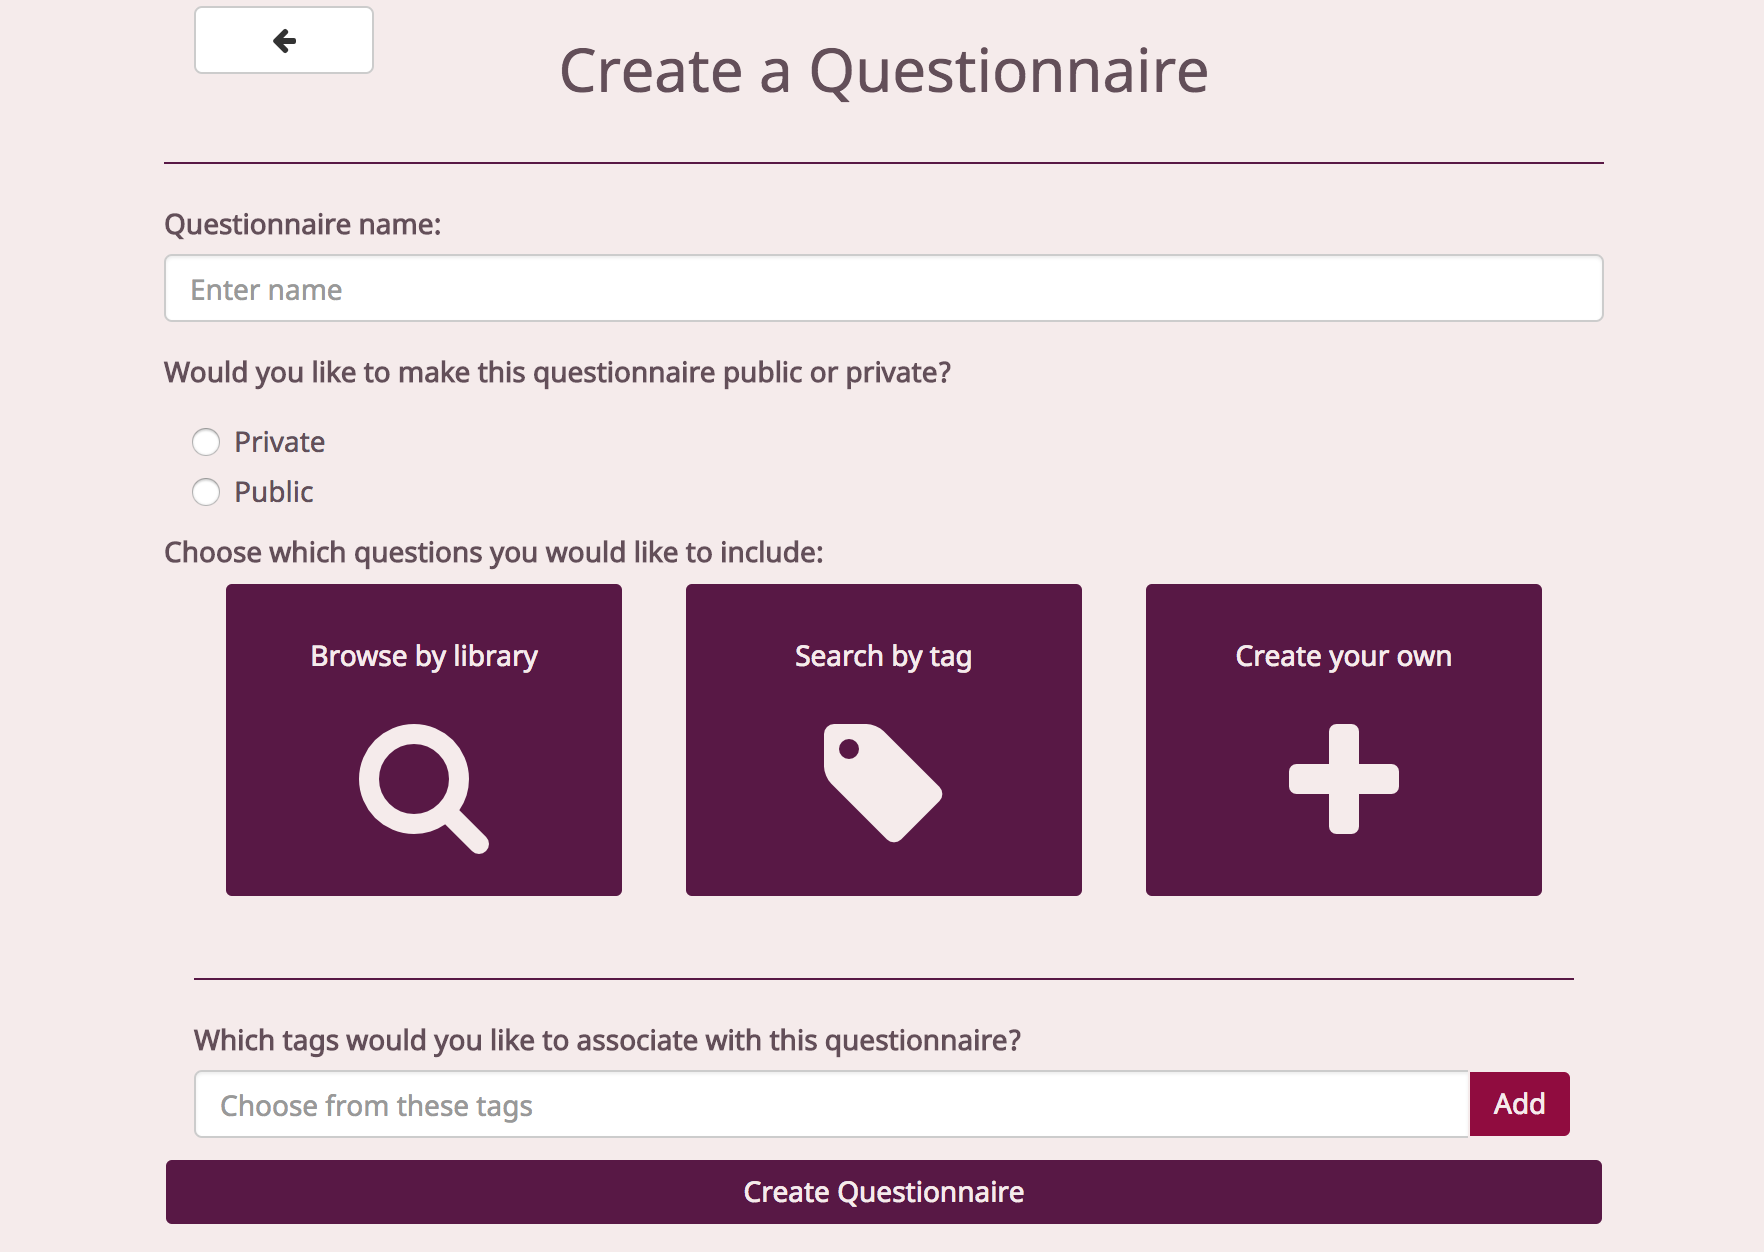
\includegraphics[scale=0.5]{Images/create.png}}
  \caption{Screenshot of the questionnaire-creation page. This first look shows the three ways physicians can add questions to questionnaires: browsing through libraries, searching by tags, and creating their own questions.} \label{Fig:create}
\end{figure}

\begin{figure}[htbp]
  \centering
  \fbox{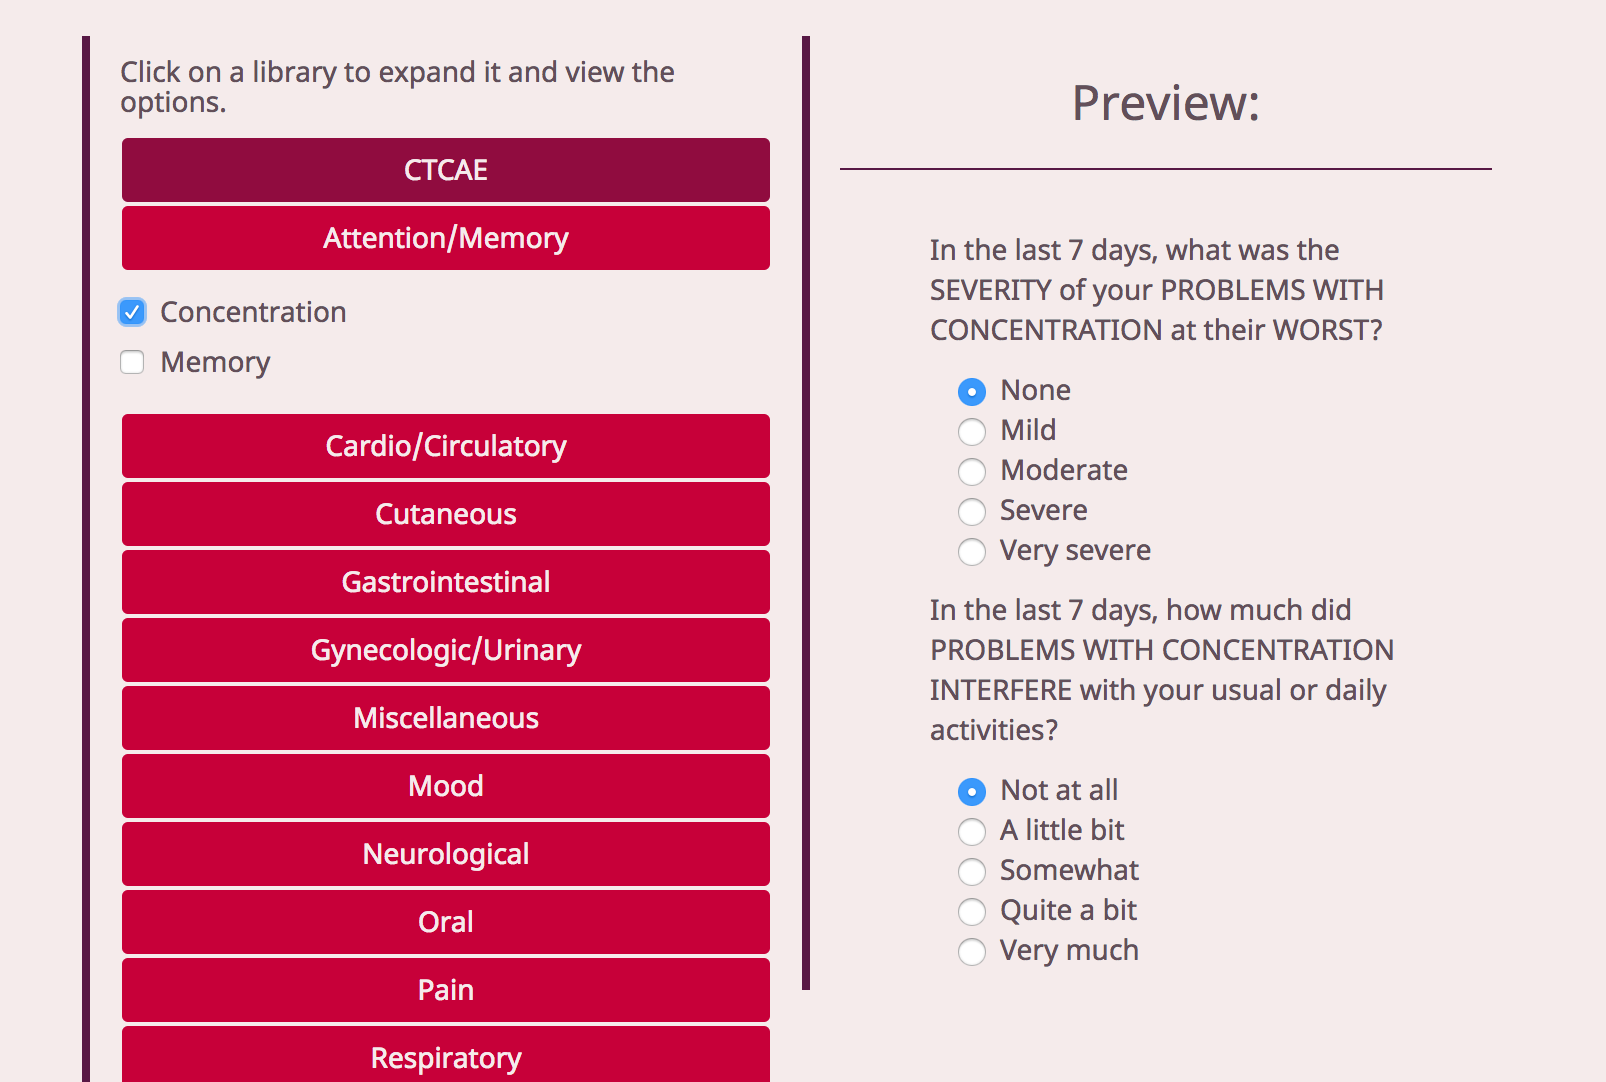
\includegraphics[scale=0.5]{Images/create_libraries.png}}
  \caption{Screenshot of the library-browsing functionality when creating questionnaires. The right-hand side shows a preview of the questionnaire.} \label{Fig:create_libraries}
\end{figure}

\begin{figure}[htbp]
  \centering
  \fbox{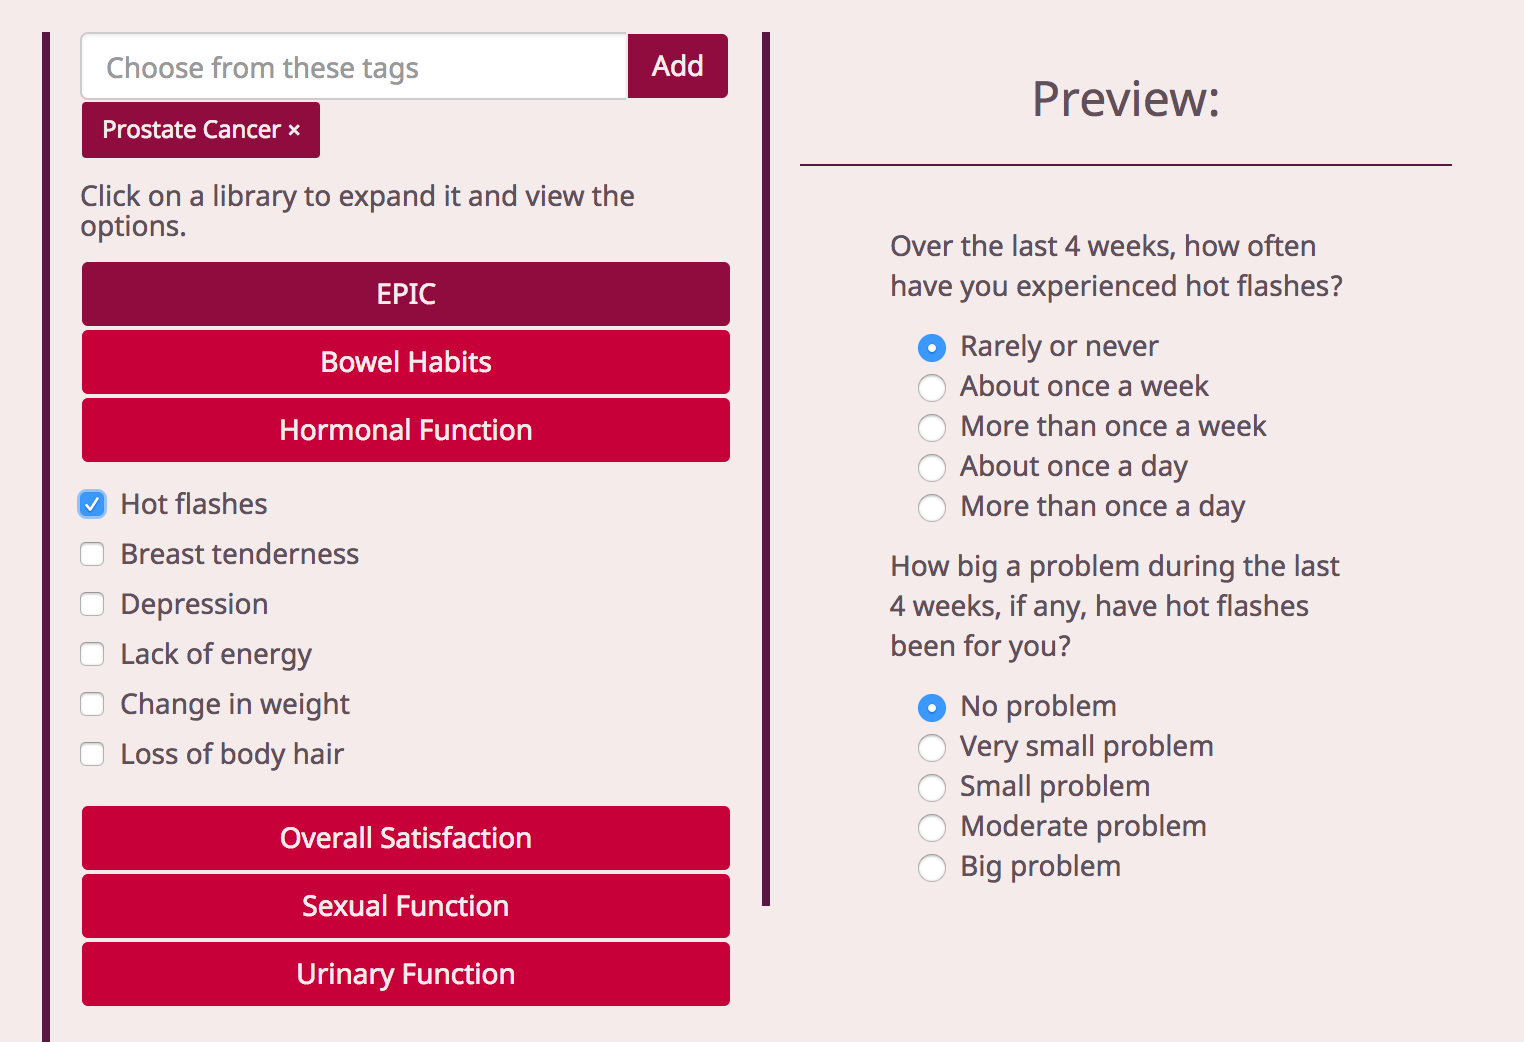
\includegraphics[scale=0.5]{Images/create_tags.png}}
  \caption{Screenshot of the tag-based search functionality when creating questionnaires. The right-hand side shows a preview of the questionnaire.} \label{Fig:create_tags}
\end{figure}

The physician may also create their own questions. Clicking the "\textit{Create your own question}" button takes them to the question bank page, as shown in \figureref{Fig:create_questionbank}, where they can both view pre-existing questions and create their own question. However, to protect the sanctity of the standardized PROM/PREM libraries, they may only add questions to their own libraries.

Lastly, before submitting their questionnaire, the physician must specify which tags will be associated with the questionnaire. These tags will then be used to locate the questionnaire in a tag-based search. This is a required field in anticipation of the numerous questionnaires that will be created, in order to make future searches more efficient.

Since the questionnaire is not in its final stage and is therefore not yet saved in \textit{QuestionnaireDB}, a version of the questionnaire is sent between the two page controllers by pushing to and popping from a global variable stack of the \textit{sharedData} service found in \textit{app.js}.



PATIENT SECTION - mention the importance of the clear divide between viewing patients' questionnaires, as well as having names written everywhere, so that a physician cannot mistake one patient's result for another patient's

%%TODO 

\chapter{Discussion and Future Work}\label{Sec:DiscussionAndFutureWork}

\section{Discussion}\label{Sec:Discussion}

The design and implementation of the questionnaire app was filled with challenges and unforeseen detours. One of these challenges was anticipating how physicians will use the app, and whether or not the flow of the forms and pages will seem natural to them. This led to frequent reshufflings of the organization of the app. 

Designing a database flexible enough to incorporate the versatility of any new question and answer type that a physician may want to create was also a significant task. The database evolved from only allowing multiple choice questions to being able to hold multiple choice, checkbox, short answer, dropdown, date, time, and linear scale questions.

Another challenge that this project faced was dealing with dynamic communication between controllers and pages. This was dealt with using AngularJS's \textit{services} functionality. We designed a shared service which provided every controller with \textit{get} and \textit{set} functions to any variable that needs to be shared between controllers. Moreover, navigating between pages proved to be awkward, with controller initializations requiring specific data being made available at specific times. This issue will need to be further addressed in the future.

Lastly, the implementation of the app needed to make it as safe as possible to use. This meant making sure that a physician can not easily accidentally mistake one patient's questionnaire results with another patient's, and creating a clear divide between patients. We dealt with this requirement by displaying each patient's list of questionnaires on an individual page unique to that patient, and making sure the patient's name is displayed on every page that is unique to them.

\section{Future Work}

While many of the desired features and functionalities of the app were successfully implemented, several remain to be done.

Opal was developed at the McGill University Health Centre (MUHC) in Quebec. As such, the questionnaire app will need to be supported in both French and English. This was left as a future task.

Opal uses \textit{OnsenUI} to format its content. As mentioned above, the questionnaire app as it stands uses very rudimentary (and inefficient) navigation between pages. A logical next step would be to integrate in \textit{OnsenUI} in order to improve the navigation through the app.

The current version of the app is a prototype, and was therefore designed without the use of ISO design standards. However, it is crucial that medical software follow standards that work to minimize human mistakes, therefore future versions should incorporate these standards. Moreover, the app should be analyzed by a human factors expert prior to deployment.

Lastly, there is also much to be done in terms of error handling and SQL sanitization.

\chapter{Conclusion}\label{Sec:Conclusion}

This project aimed to increase the versatility and usability of Opal's PRO questionnaire feature. After identifying the requirements of a questionnaire app, we implemented a database and an app to meet those goals. The current app has several new and useful features, such as the creation and editing of custom questionnaires and questions by physicians. However, much remains to be done before the app can be deployed. We look forward to seeing those changes implemented and the app launched.


%put citations here that you want to show up in your bibliography
%without mentioning them in your text.   Not generally a good idea,  but
%useful while writing drafts. In this case the '*' means that 
%all entries in sample.bib are included.
% NORMALLY you will comment the following line out for your final version
%\nocite{*}

\clearpage % start bib on new page
\bibliographystyle{plain}
\bibliography{jolly}
% pdflatex paper.tex; bibtex paper; pdflatex paper.tex; pdflatex paper.tex

% appendices come after the bibliography, each one starts with \chapter
\appendix

\chapter{Organization of Pages}\label{Sec:Org}

\begin{table}[htbp]
  \centering
  \footnotesize\sffamily
  \begin{tabular}{|| l | l ||}
    \hline\hline
    \textbf{Page}  &  \textbf{URL}\\
    \hline
    Home  & \code{/}  \\
    Create  & \code{/create/}  \\
    View Questionnaires  & \code{/questionnaires/}  \\
    View Questionnaire  & \code{/questionnaires/read/}  \\
    Edit Questionnaire  & \code{/questionnaires/edit/}  \\
    Question Bank  & \code{/questionbank/}  \\
    View Patients  & \code{/patients/}  \\
    View Patient's Questionnaires  & \code{/patients/patient/}  \\
    View Patient's Questionnaire  & \code{/patients/patient/questionnaire/}  \\
    \hline\hline
  \end{tabular}
  \caption{URLs} \label{Tab:URLs}
\end{table}

\begin{table}[htbp]
  \centering
  \footnotesize\sffamily
  \begin{tabular}{|| l | l ||}
    \hline\hline
    \textbf{Page}  &  \textbf{URL}\\
    \hline
    Home  & \code{home.html}  \\
    Create  & \code{ |--- create.html}  \\
    View Questionnaires  & \code{ |--- questionnaires.html}  \\
    View Questionnaire  & \code{ \hspace{.5cm} |--- read.html}  \\
    Edit Questionnaire  & \code{ \hspace{.5cm} |--- edit.html}  \\
    Question Bank  & \code{ |--- question-bank.html}  \\
    View Patients  & \code{ |--- patients.html}  \\
    View Patient's Questionnaires  & \code{ \hspace{.5cm}	|--- patient.html}  \\
    View Patient's Questionnaire  & \code{ \hspace{1.4cm}|--- patient-questionnaire.html}  \\
    \hline\hline
  \end{tabular}
  \caption{Views} \label{Tab:Views}
\end{table}

\begin{table}[htbp]
  \centering
  \footnotesize\sffamily
  \begin{tabular}{|| l | l ||}
    \hline\hline
    \textbf{Page}  &  \textbf{URL}\\
    \hline
    Home  & \code{HomeController}  \\
    Create  & \code{ |--- CreateController}  \\
    View Questionnaires  & \code{ |--- QuestionnairesController}  \\
    View Questionnaire  & \code{ \hspace{.5cm} |--- ReadController}  \\
    Edit Questionnaire  & \code{ \hspace{.5cm} |--- EditController}  \\
    Question Bank  & \code{ |--- QuestionBankController}  \\
    View Patients  & \code{ |--- PatientsController}  \\
    View Patient's Questionnaires  & \code{ \hspace{.5cm}	|--- PatientController}  \\
    View Patient's Questionnaire  & \code{ \hspace{1.4cm}|--- PatientQuestionnaireController}  \\
    \hline\hline
  \end{tabular}
  \caption{Controllers} \label{Tab:Controllers}
\end{table}

\newpage
\chapter{Pellentesque habitant
  morbi tristique senectus et netus et malesuada fames ac turpis
  egestas}

\begin{figure}
  \centering
  \fbox{
\includegraphics[width=2in]{Images/red_corps_castle2}}
  \caption{Yet Another Castle In Appendix} \label{Fig:castle2}
\end{figure}

\end{document}
